% Polished Comparative Evaluation section (proofread by Claude). Original text is in main-original.tex.
\section{Comparative Evaluation}
\label{sec:eval}
\subsection{Setup and Metrics}
\label{sec:setup}
We evaluate BrickForma against BrickGPT and BrickNet on 525 shared prompts spanning 21 categories and five description levels (105 prompts per level). Scoring one delivered output per system and prompt yields 1,575 LDraw exports. To isolate the geometric quality of the learned model before solver intervention, the main benchmark scores every delivered raw BrickForma export, including incomplete drafts; Appendix~\ref{app:eval} reports the refinement diagnostic separately.

\emph{Text--image alignment.}
Each export is rendered in a uniform yellow material from eight $512{\times}512$ orthographic views, spaced $45^\circ$ apart in azimuth at $25^\circ$ elevation. Each alignment score takes the maximum over views and is then averaged across prompts. VQAScore~\cite{vqascore} is the first-token probability of \textquotedblleft Yes\textquotedblright\ under Qwen2.5-VL-7B-Instruct~\cite{qwen25vl}; PE~\cite{pe} is the cosine similarity between normalized image and text embeddings; and SigLIP2~\cite{siglip2} is the sigmoid of the image--text logit.

\emph{Invalid placements.}
For an export with $n$ placements in file order, let $I_i$ indicate whether placement $i$ violates BrickNet's inset collision kernel~\cite{bricknet} given the preceding placements. We report the mean per-export invalid-placement ratio $P_{\mathrm{inv}}=n^{-1}\sum_{i=1}^{n}I_i$.

\subsection{Main Results}
\begin{table}[t]
\centering\small
\setlength{\tabcolsep}{3pt}
\begin{tabular}{lrrrr}
\toprule
System & $P_{\mathrm{inv}}\downarrow$ & VQAScore $\uparrow$ & PE $\uparrow$ & SigLIP2 $\uparrow$ \\
\midrule
BrickForma & 0.79\% & \textbf{0.0866} & \textbf{0.1568} & \textbf{0.0448} \\
BrickGPT & \textbf{0.00\%} & 0.0666 & 0.1440 & 0.0194 \\
BrickNet & 18.42\% & 0.0201 & 0.1187 & 0.0011 \\
\bottomrule
\end{tabular}
\caption{Mean scores on the 525 shared prompts. BrickForma is scored on its delivered raw outputs. Bold marks the best mean.}
\label{tab:main}
\end{table}

Across all 525 prompts, BrickForma's raw outputs achieve the highest mean VQAScore (0.0866), PE (0.1568), and SigLIP2 (0.0448) (Table~\ref{tab:main}), outperforming BrickGPT on 384, 337, and 327 prompts, respectively. All six paired alignment comparisons remain statistically significant after Holm correction (Appendix~\ref{app:eval}). For placement validity, BrickGPT achieves the lowest mean $P_{\mathrm{inv}}$ (0.00\%) through physics-aware rollback, followed by BrickForma (0.79\%) and BrickNet (18.42\%); 525, 331, and 139 of their outputs, respectively, contain no invalid placement (Figure~\ref{fig:comparison-zero-invalid}). Figures~\ref{fig:comparison-means} and~\ref{fig:comparison-distributions} show the pooled means and score distributions.

\paragraph{Comparison with the untuned backbone.}
To measure the effect of parametric supervision, and thus to address \textbf{(Q2)}, we compare against untuned Qwen3-1.7B on 260 matched prompts, assigning zero alignment scores whenever it fails to produce a scorable layout. Mean VQAScore, PE, and SigLIP2 rise from 0.0008, 0.0354, and 0.0014 for the untuned backbone to 0.0649, 0.1564, and 0.0328 for raw BrickForma before geometric refinement (Appendix~\ref{app:eval}).

\subsection{Performance across Description Levels}
\begin{table*}[t]
\centering\small
\setlength{\tabcolsep}{3pt}
\begin{tabular}{lrrlrrrr}
\toprule
Level & $n$ & Words & System & $P_{\mathrm{inv}}\downarrow$ & VQAScore $\uparrow$ & PE $\uparrow$ & SigLIP2 $\uparrow$ \\
\midrule
L1 & 105 & 13.6 & BrickForma & 0.48\% & \textbf{0.1539} & \textbf{0.1388} & \textbf{0.0158} \\
 &  &  & BrickGPT & \textbf{0.00\%} & 0.1296 & 0.1302 & 0.0087 \\
 &  &  & BrickNet & 18.59\% & 0.0346 & 0.1051 & 0.0005 \\
\midrule
L2 & 105 & 26.4 & BrickForma & 0.69\% & \textbf{0.1264} & \textbf{0.1465} & \textbf{0.0291} \\
 &  &  & BrickGPT & \textbf{0.00\%} & 0.0938 & 0.1338 & 0.0206 \\
 &  &  & BrickNet & 18.35\% & 0.0394 & 0.1030 & 0.0008 \\
\midrule
L3 & 105 & 37.5 & BrickForma & 0.98\% & \textbf{0.1179} & \textbf{0.1477} & \textbf{0.0508} \\
 &  &  & BrickGPT & \textbf{0.00\%} & 0.0863 & 0.1415 & 0.0178 \\
 &  &  & BrickNet & 22.98\% & 0.0209 & 0.1113 & 0.0012 \\
\midrule
L4 & 105 & 52.5 & BrickForma & 1.08\% & \textbf{0.0192} & \textbf{0.1780} & \textbf{0.0738} \\
 &  &  & BrickGPT & \textbf{0.00\%} & 0.0148 & 0.1605 & 0.0338 \\
 &  &  & BrickNet & 17.24\% & 0.0025 & 0.1376 & 0.0011 \\
\midrule
L5 & 105 & 78.8 & BrickForma & 0.75\% & \textbf{0.0157} & \textbf{0.1730} & \textbf{0.0543} \\
 &  &  & BrickGPT & \textbf{0.00\%} & 0.0086 & 0.1542 & 0.0162 \\
 &  &  & BrickNet & 14.95\% & 0.0030 & 0.1363 & 0.0020 \\
\bottomrule
\end{tabular}
\caption{Mean scores by description level. Each level contains 105 prompts per system; Words is the mean English word count of the prompts. Bold marks the best mean.}
\label{tab:level-results}
\end{table*}

Addressing \textbf{(Q1)}, BrickForma leads on all three alignment metrics at every description level, from concise L1 requests to detailed L5 specifications (Table~\ref{tab:level-results} and Figure~\ref{fig:comparison-levels}). At L1, its mean VQAScore is 0.1539, compared with 0.1296 for BrickGPT and 0.0346 for BrickNet; BrickGPT keeps $P_{\mathrm{inv}}$ at 0.00\% at every level. Figure~\ref{fig:gallery} shows qualitative L1 and L2 examples under matched rendering conditions.

\begin{figure*}[t]
\centering
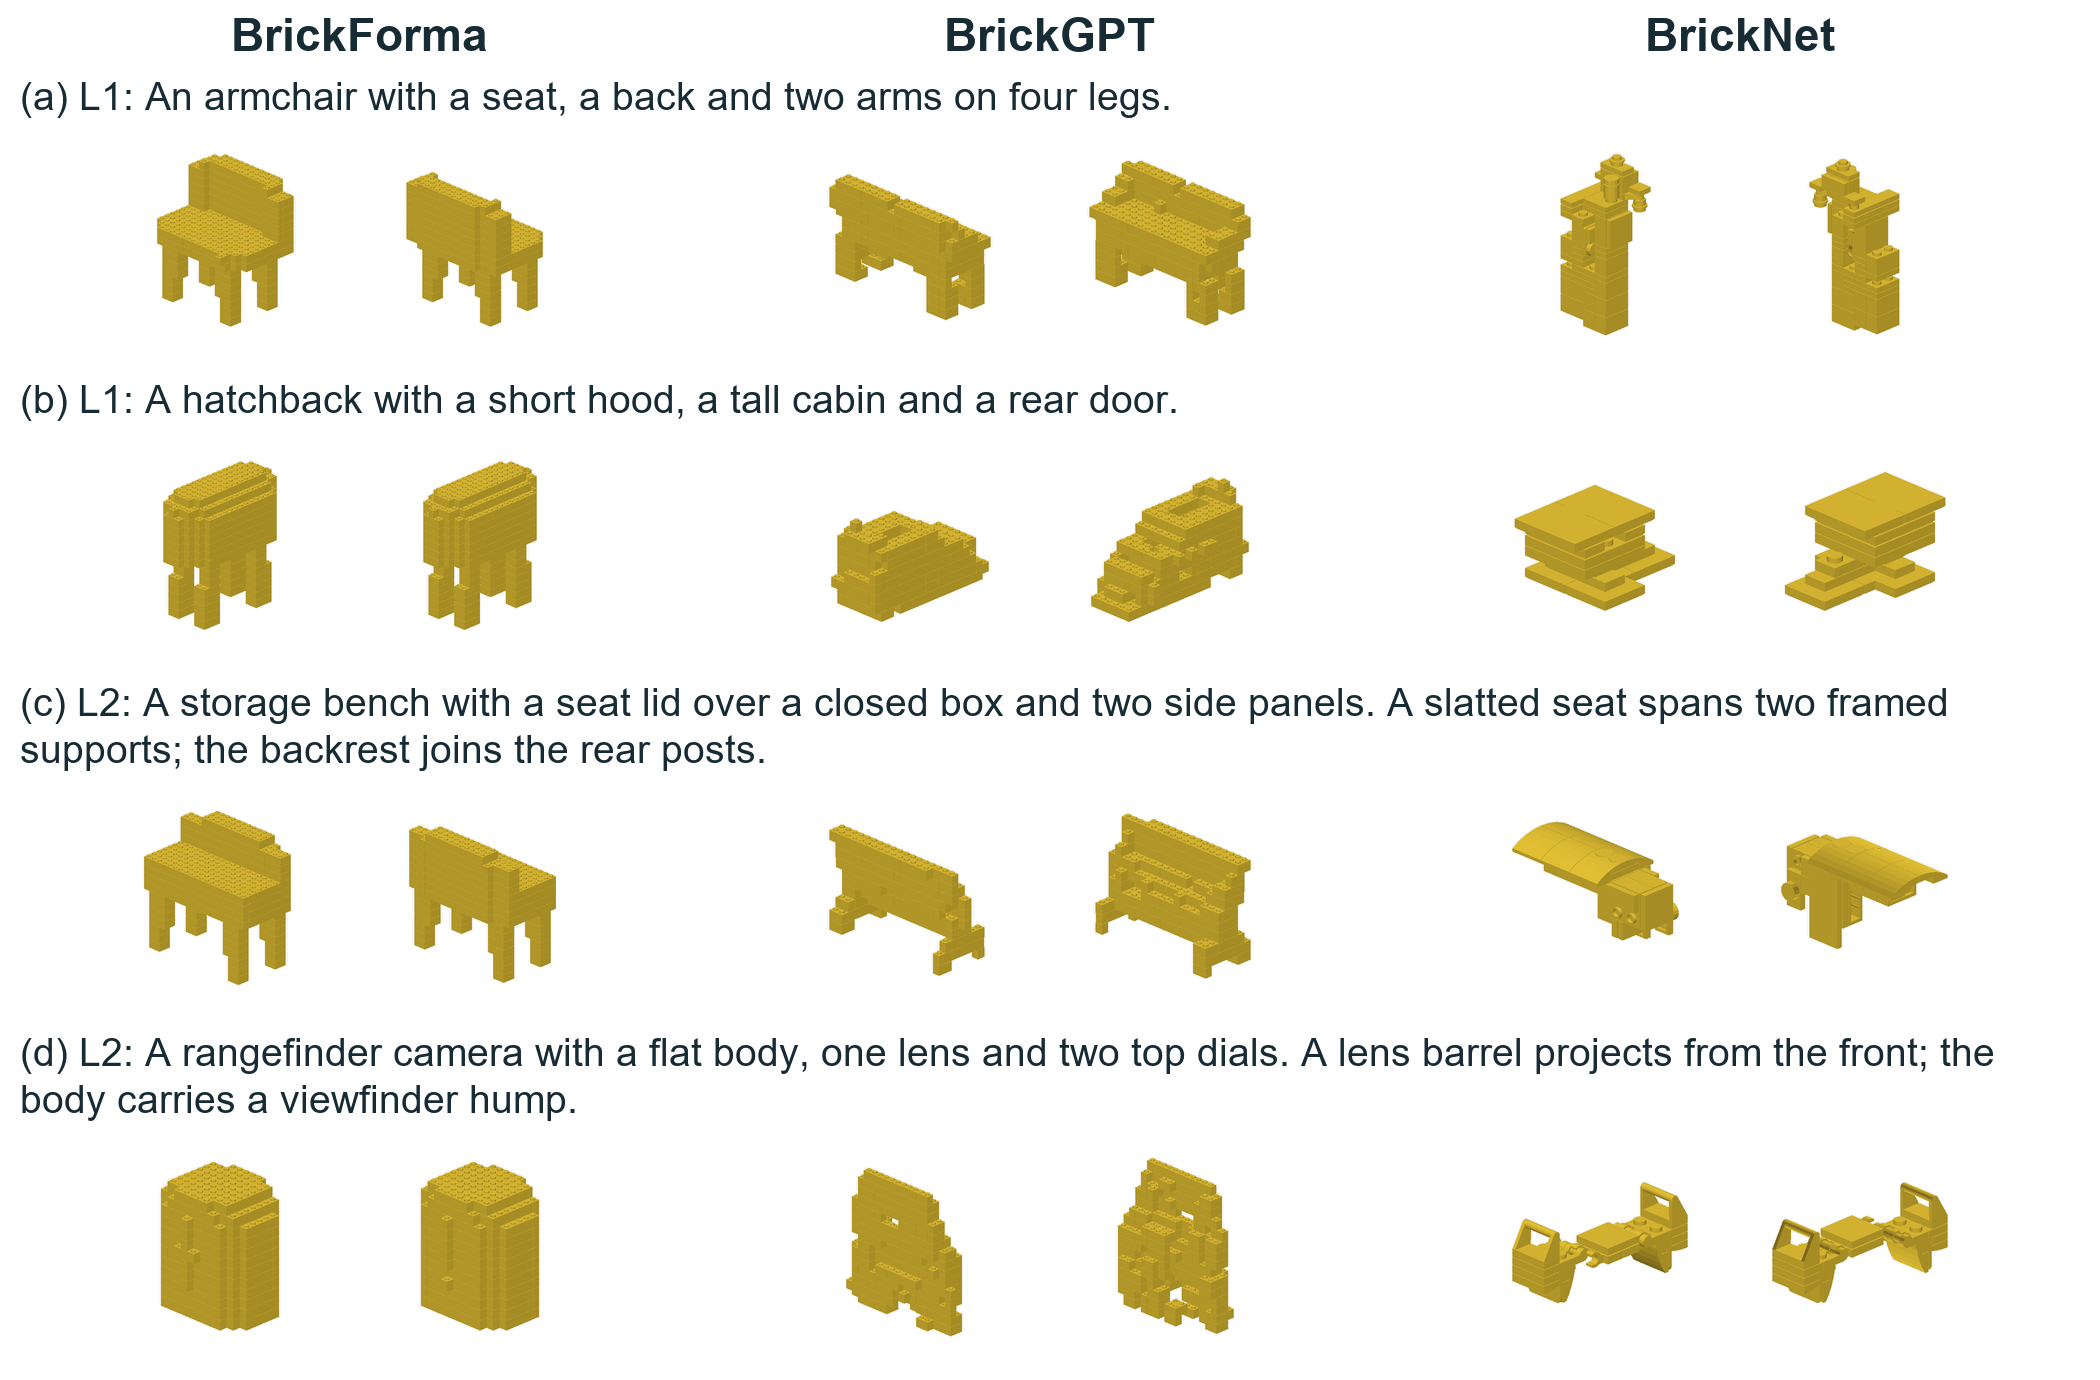
\includegraphics[width=\textwidth]{figures/matched_short_prompts_20261116.png}
\caption{Four examples from the matched evaluation, with the same prompts, render settings, and azimuths ($45^\circ$ and $225^\circ$) for all systems. The highest VQAScore goes to BrickForma for the armchair and the storage bench, to BrickGPT for the hatchback, and to BrickNet for the camera.}
\label{fig:gallery}
\end{figure*}


\subsection{Raw versus Refined Outputs}
\begin{table}[t]
\centering
\small
\begin{tabular}{lrr}
\toprule
Metric & Raw & Refined \\
\midrule
$P_{\mathrm{inv}}$ $\downarrow$ & 0.1897\% & 0.0000\% \\
VQAScore $\uparrow$ & 0.2065 & 0.2071 \\
PE $\uparrow$ & 0.1858 & 0.1859 \\
SigLIP2 $\uparrow$ & 0.1379 & 0.1261 \\
Mean parts & 178.7 & 421.2 \\
\bottomrule
\end{tabular}
\caption{Raw versus refined BrickForma outputs on 110 pairs from the earlier comparison. Each pair shares the same prompt, model identifier, and caption.}
\label{tab:raw-refined}
\end{table}

To quantify the effect of exact-cover reconstruction, we examine 110 raw/refined pairs from an earlier 114-prompt comparison; each pair shares the same prompt and model identifier (Table~\ref{tab:raw-refined}). Refinement eliminates invalid placements ($P_{\mathrm{inv}}$ drops from 0.1897\% to 0.0000\%) and raises the mean part count from 178.7 to 421.2. VQAScore and PE remain essentially unchanged, whereas SigLIP2 decreases from 0.1379 to 0.1261.

\subsection{Geometric Refinement Audit}
\label{sec:diagnostics}
Defining stud contacts as footprint overlaps between adjacent layers, we map the same 110 pairs onto a grid with a 20\,LDU horizontal pitch and a 24\,LDU layer height, and align each export to a common occupied-cell origin. All 110 pairs keep identical occupied voxel unions after translation, while the number of single-component assemblies rises from 18 to 110 and the number of overlap-free layouts from 100 to 110 (Table~\ref{tab:export-audit}).
\begin{table}[t]
\centering\small
\begin{tabular}{@{}lrr@{}}
\toprule
Export measure & Raw & Refined \\
\midrule
Single stud component & 18/110 & 110/110 \\
Mean stud components & 4.29 & 1.00 \\
No body-cell overlap & 100/110 & 110/110 \\
\midrule
\multicolumn{3}{@{}l@{}}{Equal voxel unions after translation: 110/110} \\
\bottomrule
\end{tabular}
\caption{Export audit of the 110 matched raw/refined pairs from the earlier comparison. Voxel unions are compared after translation normalization.}
\label{tab:export-audit}
\end{table}


In the separate 525-prompt diagnostic run, only 46 raw drafts form a single stud component, whereas all 525 final layouts are single stud-connected components that preserve their target voxel unions after the recovery procedure (Appendix~\ref{app:eval}).

\subsection{Evaluation Boundaries}
Our benchmark compares delivered exports from systems that differ in inference settings and part libraries. Description levels differ in both semantic detail and token length, so PE truncates 121 prompts and SigLIP2 truncates 209 (Appendix~\ref{app:eval}). Uniform yellow rendering isolates geometric form and layout but does not assess color fidelity. Finally, the paired refinement audit covers only delivered pairs, so unsuccessful solver attempts are excluded from its denominator.
